\documentclass{article}
\usepackage[letterpaper, margin=1in]{geometry}
\usepackage[pdftex]{graphicx}
\usepackage[utf8]{inputenc}
\usepackage{tikz, pgfplots, wrapfig, amssymb, array, mathtools, enumitem, circuitikz, physics, parskip, hyperref}
\usepackage{tkz-euclide}
\usepackage{titlesec}
\usepackage{lipsum}
\usepackage[english]{babel}
\usepackage{amsmath, amsthm}
\usepackage{fancyhdr}
\usepackage{xcoffins}
\usepackage{tcolorbox}
\usepackage{../local}

\pgfplotsset{compat=1.17}

\title{Physics 5C Homework}
\author{Yutong Du}


\begin{document}

\maketitle 

\section*{Collaborators}

I worked primarily with \textbf{Andrew Binder} to complete this homework. Credit to him for the \tikz code in Problem 5. 

\section*{Problem 1}

This question is about a discrete probability distribution known as the \textbf{Poisson distribution}. Let $x$ be a discrete random variable that can take values $0, 1, 2, \dots$. A quatity $x$ is said to be Poisson distributed if the probability $P(x)$ of obtaining $x$ is


\[ P(x) = \frac{e^{-m} m^x}{x!}\]

where $m$ is a particular number (which we will show in part (b) of this exercise is the mean value of $x$). 



\begin{enumerate}[label=(\alph*)]
    \item Show that $P(x)$ is a well-behaved probability distribution in the sense that
    
    \[ \sum_{x= 0}^\infty P(x) = 1\] 

    \begin{solution}
        It helps to expand out a couple terms from the summation:

        \begin{align*}
            \sum P(x) &= e^{-m} + me^{-m} + \frac{e^{-m} m^2}{2!} + \dots\\
            &= e^{-m}\left(1 + m + \frac{m^2}{2} + \dots \right)\\
        \end{align*}

        What we notice is that the term in the parentheses is the taylor expansion for $e^{m}$, so we have $\sum P(x) = e^{-m}e^{m} = 1$.

        A quick comment on why this result is important: if it had not been the case that $\sum P(x) = 1$, then it would mean that the probability for any of the possibilities to happen is greater than 1, which is nonphysical.
    \end{solution}

    \item Show that the mean value of the probability distribution is $\mean{x} = \sum_{x = 0}^\infty = m$
    
    \begin{solution}
        Again, it helps to expand here:

        \begin{align*}
            \sum_{x = 0}^\infty xP(x) &= me^{-m} + 2\frac{m^2e^{-m}}{2!} + \dots + n\frac{{m^n}e^{-m}}{n!}\\
            &= e^{-m} \left(me^{-m} + \frac{2m^2}{2!} + \dots + \frac{nm^n}{n!}\right)
        \end{align*}

        Here we can rewrite the general term $\frac{nm^n}{n!} = m \frac{m^{n-1}}{(n-1)!}$, so we can factor $m$:

        \begin{align*}
            \sum_{x = 0}^\infty xP(x) &= me^{-m} \left(1 + m + \frac{m^2}{2} + \dots \right)\\
            &= m e^{-m}e^{m} = m
        \end{align*}

        Just like part (a), the term in the parentheses is just the taylor expansion for $e^{m}$, which justifies the last step.
    \end{solution}


    \item The text was too long for me to type it out, but here's my solution:
    
    \begin{solution}
        From the table, we know that the mean is 
        
        
        \[\mean{x} = \frac{\sum x_if_i}{\sum x_i} = \frac{122}{200} = 0.61\]
        
        
        Since we know that the mean of the distribution must be $m$, then we know that $m = 0.61$. Now that we have $P(x)$ we need to multiply $P(x)$ by the total frequency in order to get our counts:
        
        \begin{center}
            \begin{tabular}{|l|l|}
            \hline
            $x$ & $P(x)$ \\ \hline
            0   & 108.7  \\ \hline
            1   & 66.29  \\ \hline
            2   & 20.22  \\ \hline
            3   & 4.11  \\ \hline
            4   & 0.63  \\ \hline
            5   & 0.07   \\ \hline
            6   & 0
            \end{tabular}
        \end{center}
        In reality the value we get at 6 is 0.00003, but we can effectively take this as equalling zero. Overall, the theoretical poisson distribution matches the observed values quite well.
    \end{solution}

\end{enumerate}

\pagebreak
\section*{Problem 2}

This question is about a continuous probability distribution known as the \textbf{exponential distribution}. Let $x$ be a continuous random variable that can take any value $x \ge 0$. A quantity is said to be exponentially distributed if it takes values between $x$ and $x +\dx$ with probability 

\[ P(x) dx = Ae^{-x/\lambda} \dx\]

where $\lambda$ and $A$ are constants. 

\begin{enumerate}[label = (\alph*)]
    \item Find the value of $A$ that makes $P(x)$ a well defined continuous probability distribution so that $\int_0^\infty P(x) \dx = 1$. 
    
    \begin{solution}
        Taking the integral:

        \begin{align*}
            1 &= \int_0^\infty P(x) \dx = A \int_0^\infty e^{-x/\lambda} \dx\\
            \therefore A &= \frac{1}{\int_0^\infty e^{-x/\lambda } \dx}\\
            A &= \frac{1}{-\lambda e^{-x/\lambda}\bigg|_0^\infty}
        \end{align*}

        Now evaluating the bounds, we have $x = 0 \rightarrow -\lambda$, and $x = \infty \rightarrow 0$, so we have:

        \[ A = \frac{1}{\lambda}\]

            
    \end{solution}

    \item Show that the mean value of the probability distribution is $\mean {x} = \int_0^\infty xP(x) \dx = \lambda$. 

    \begin{solution}
        We compute the integral, using the $A$ that we found before:

        \begin{align*}
            \int_0^\infty xP(x) &= \int_0^\infty x \cdot \frac{1}{\lambda}e^{-x/\lambda} \dx\\
            &= \frac{1}{\lambda} \int_0^\infty xe^{-x/\lambda} \dx\\
            &= \frac{1}{\lambda}\left[\underbrace{x(-\lambda) e^{-x/\lambda} \bigg|_0^\infty}_{= 0} + \lambda e^{-x/\lambda} \dx\right] && \text{integration by parts}\\
            &= \int_0^\infty e^{-x/\lambda} \dx \\
            &= \lambda && \text{from part (a)}
        \end{align*}
    \end{solution}


    \item Find the variance and standard deviation of this probability distribution.
    
    \begin{solution}
        Variance is defined as $\sigma_x^2 = \mean{x^2} - \mean{x}^2$. We know that $\mean x^2 = \lambda^2$ from our previous result, so all we have to do is compute $\mean{x^2}$:

        \begin{align*}
            \mean{x^2} &= \int_0^\infty x^2P(x) \dx\\
            &= \frac{1}{\lambda} \int_0^\infty x^2e^{-x/\lambda} \dx \\
            &= \frac{1}{\lambda}\left[\underbrace{x^2(-\lambda)e^{-x/\lambda}\bigg|_0^\infty}_{= 0} + \lambda \int_0^\infty 2xe^{-x/\lambda} \dx\right] && \text{integration by parts}\\
            &= 2\int_0^\infty xe^{-x/\lambda} \dx
        \end{align*} 

        We've computed this integral before in part (a), but with a prefactor of $-\frac{1}{\lambda}$, thus, rearranging, we get

        \[ 2\int_0^\infty xe^{-x/\lambda} \dx = \boxed{2\lambda^2}\]


        Thus, we now complete the problem: $\sigma_x^2 = 2\lambda^2 - \lambda^2 = \lambda^2$, and the standard deivation is $\sqrt{\sigma_x^2} = \lambda$.
    \end{solution}
\end{enumerate}

\pagebreak
\section*{Problem 3}

If $\theta$ is a continuous distribution random variable which is uniformly distributed between 0 and $\pi$, write down an expression for $P(\theta)$. Hence find the value of the following averages:


\begin{solution}

    Since $\theta$ is distributed between $0$ and $\pi$, we know that 

    \[ \int_0^\pi P(\theta) \ \mathrm d \theta= 1\]

    And since the distribution is uniform, then $P(\theta)$ should be a constant for all $\theta$. Therefore we have $P(\theta) = \frac{1}{\pi}$ for all $\theta$.
\end{solution}
\begin{enumerate}[label=(\alph*)]
    \item $\mean{\theta}$
    
    \begin{solution}
        \begin{align*}
            \mean{\theta} &= \int_0^\pi \theta P(\theta) \dd \theta\\
            &= \frac{1}{\pi} \int_0^\pi \theta \dd \theta \\
            &= \frac{1}{\pi} \frac{\theta^2}{2}\bigg|_0^\pi\\
            &= \frac{\pi}{2}
        \end{align*}

        This makes sense, since this value is exactly in between $0$ and $\pi$.
    \end{solution}
    
    
    \item $\mean{\theta - \frac{\pi}{2}}$
    
    \begin{solution}
        By linear transformation we have $\mean{\theta - \frac{\pi}{2}} = \mean{\theta} - \frac{\pi}{2}$ so using our result from the previous part 

        \[ \mean{\theta - \frac{\pi}{2}} = \boxed{0}\]

        This makes sense, by linearity.
    \end{solution}


    \item $\mean{\theta^2}$:
    
    \begin{solution}
        Since $\mean{f(x)} = \int f(x) P(x) \dx$, then we have

        \begin{align*}
            \mean{\theta^2} &= \int_0^\pi \theta^2 \frac{1}{\pi} \dd \theta\\
            &= \frac{1}{\pi}\frac{\theta^3}{3}\bigg|_0^\pi\\
            &= \frac{\pi^2}{3}
        \end{align*}

        This result makes sense since $\sigma_\theta^2$ is nonzero, so this value must be different than $\mean{\theta}^2$. I cannot justify why the precise value is $\frac{\pi^2}{3}$ aside from saying that it comes from the integral.
    \end{solution}


    \item $\mean{\theta^n}$
    
    \begin{solution}
        Same thing as part (c) here:

        \begin{align*}
            \mean{\theta^n} &= \int_0^\pi \theta^n \frac{1}{\pi} \dd \theta \\
            &= \frac{1}{\pi} \frac{\theta^{n+1}}{n+1}\\
            &= \frac{\pi^{n}}{n + 1}
        \end{align*}

        This is a natural generalization of part (c).
    \end{solution}


    \item $\mean{\cos \theta}$
    
    \begin{solution}
        \begin{align*}
        \mean{\cos \theta} &= \frac{1}{\pi} \int_0^\pi \cos \theta  \dd \theta \\
        &= \frac{1}{\pi} \sin \theta \bigg|_0^\pi\\
        &= 0
        \end{align*}

        This makes sense since on the interval from $0$ to $\pi$, $0$ is the average value of cosine over that interval.
    \end{solution}


    \item $\mean{\sin \theta}$
    
    \begin{solution}
        \begin{align*}
            \mean{\sin\theta} &= \frac{1}{\pi} \int_0^\pi \sin \theta \dd \theta\\
            &= \frac{1}{\pi}(- \cos \theta)\bigg|_0^\pi\\
            &= -\frac{1}{\pi} (-1 -1)\\
            &= \frac{2}{\pi}
        \end{align*}

        This result makes sense in more or less the same way the previous result makes sense. The mean value of $\sin \theta$ over $[0, \pi]$ is nonzero, and so we expect a nonzero result.
    \end{solution}


    \item $\mean{\left|\cos \theta\right|}$
    
    \begin{solution}
        \begin{align*}
            \mean{\sin \theta} &= \frac{1}{\pi} \int_0^\pi |\cos \theta| \dd \theta\\
            &= \frac{2}{\pi} \int_0^{\frac{\pi}{2}}\cos \theta \dd \theta\\
            &= \frac{2}{\pi} \sin \theta \bigg|_0^\frac{\pi}{2}\\
            &= \frac{2}{\pi}
        \end{align*}

        We expect this result to be the same as that of $\sin \theta$, since the curves are the same, since the negative part of $\cos \theta$ is reflected about the $x$ axis, becoming positive.
    \end{solution}

    \item $\mean{\cos^2 \theta}$
    
    \begin{solution}
        \begin{align*}
            \mean{\cos^2 \theta} &= \frac{1}{\pi} \int_0^\pi \cos^2 \theta \dd \theta\\
            &= \frac{1}{\pi} \int_0^\pi \frac{\cos(2\theta)+1}{2} \dd \theta \\
            &= \frac{1}{2\pi}\left[\frac{1}{2} \sin (2\theta) + \theta\right]_0^\pi\\
            &= \frac{1}{2}
        \end{align*}

        This result makes sense when combined with part (i) and (j), since we should get that $\mean{\cos^2 \theta + \sin^2 \theta} = \mean{\cos^2 \theta} + \mean{\sin^2 \theta} = 1$.
    \end{solution}

    \item $\mean{\sin^2 \theta}$
    
    \begin{solution}
        \begin{align*}
            \mean{\sin^2 \theta} &= \frac{1}{\pi} \int_0^\pi \sin^2 \theta \dd \theta\\
            &= \frac{1}{\pi} \left(\int_0^\pi 1 \dd \theta - \int_0^\pi \cos^2\theta \dd \theta \right)\\
            &= \frac{1}{\pi} \left(\pi - \frac{\pi}{2}\right)\\
            &= \frac{1}{2}
        \end{align*}

        This result makes sense, since we know that $\mean{\cos^2\theta + \sin^2\theta}= 1$, and knowing that $\mean{\cos^2\theta} = \frac{1}{2}$, it must follow that $\mean{\sin^2\theta} = \frac{1}{2}$.
    \end{solution}


    \item $\mean{\cos^2 \theta + \sin^2 \theta}$

    \begin{solution}
    Since this quantity is always equal to 1, then $\mean{\cos^2\ \theta + \sin^2 \theta} = 1$. This makes sense, since this value is always equal to 1 over the interval $[0, \pi]$.

    \end{solution}
\end{enumerate}


\pagebreak
\section*{Problem 4}

In experimental physics, it is important to repeat measurements. Assuming that errors are random, show that if the error in making a single measurement of quantity $X$ is $\Delta$, the error obtained after using $n$ measurements $\Delta/\sqrt{n}$


\begin{solution}
    Let $Y = X_1 + \dots + X_n$. To calculate the error after $n$ measurements, we calculate $\sigma_Y$. To do that, we calculate variance:

    \[ \sigma_Y^2 = \mean{Y^2} - \mean{Y}^2\]


    We can calculate each of the terms on the right separately:

    \begin{align*}
        \mean{Y^2} &= \mean{(X_1 + \dots + X_n)^2}\\
        &= \mean{X_1}^2 + \mean{X_2}^2 + \dots + \mean{X_n}^2 + \mean{X_1}\mean{X_2} + \text{(very many cross terms)}\\
        \mean{Y}^2 &= \mean{\sum_n X_i}^2\\
        &= \mean{X_1^2 + X_2^2 + \dots + X_n^2 + X_1X_2 + \text{more cross terms}}^2\\
        &= \mean{X_1}^2 + \mean{X_2}^2 + \dots + \mean{X_1}\mean{X_2} + \dots
    \end{align*}

    Notice that the cross terms in $\mean{Y^2}$ and $\mean{Y}^2$ cancel out pefectly after subtraction. Likewise, notice that the remaining terms can be grouped as $\mean{X_i^2} - \mean{X_i}^2 = \Delta^2$, and we have $n$ of these terms so we obtain:

    \[ \sigma_Y^2 = n \sigma_X^2\]

    Now note that since $Y = X_1 + \dots + X_n$, we need to divide this by $n$ to obtain the quantity we want. Since each term is then divided by $n$, we simply have an overall factor of $\frac{1}{n^2}$ that is factored out. Thus:

    \[ \sigma_{Y/n}^2 = \frac{n \sigma_X^2}{n^2}\]

    And thus

    \[ \sigma_{Y/n} = \frac{\sigma_X}{\sqrt{n}} = \frac{\Delta}{\sqrt{n}}\]



    % Let $Y = nX$. When we are asked to the error obtained after using $n$ measurements, we are thus asking for the standard deviation of $Y$. To compute this, we calculate variance, then take the square root:

    % \[ \sigma_Y^2 = \mean{Y^2} - \mean{Y}^2\]

    % From our earlier equation we know that $\mean{Y} = n\mean{X}$, by linearity. Thus, we have $\mean{Y}^2 = n^2\mean{X}^2$. Now we calculate $\mean{Y^2}$ 

    % \begin{align*}
    %     \mean{Y^2} &= \mean{n^2X^2}\\
    %     &= n^2 \mean{X^2}
    % \end{align*}

    % Thus, we have:

    % \[ \sigma_Y^2 = n^2\mean{X^2} - n^2 \mean{X}^2 = n^2 \sigma_x^2\]

    
\end{solution}


\pagebreak
\section*{Problem 5}
A system comprises of $N$ states, which can have energy $0$ or $\Delta$. Show that the number of ways $\Omega(E)$ of arranging the total system to have energy $E = r\Delta$ (where $r$ is an integer) is given by 

\[ \Omega(E) = \frac{N!}{r!(N - r)!}\] 

Now remove a small amount of energy $s\Delta$ from the system, where $s \ll r$. Show that 

\[ \Omega(E - \epsilon) \approx \Omega(E) \frac{r^s}{(N - r)^s}\]

and hence show that the system has temperature $T$ given by 

\[ \frac{1}{k_BT} = \frac{1}{\Delta} \ln \left( \frac{N - r}{r}\right)\]

Sketch $k_BT$ as a function of $r$ from $r = 0$ to $r = N$ and explain the result.

\begin{solution}
    We have $N$ particles, and we want to select $r$ of them. The number of ways we can do this is $\frac{N!}{(N - r)!}$. However, since this selection should not care about the order in which the particles are arranged, we need to divide by a further $r!$ in order to remove this excessive counting. Thus, our formula becomes:

    \[ \Omega(E) = \frac{N!}{r!(N- r)!}\]

    For the second part of the problem: we make the argument that in the case when these values get large, we can simplify the factorial to a simple exponential. Specifically, we can approximate $n! \approx n^n$, arguing that the cross terms are substantially smaller than the leading term. Thus, 

    \[ \Omega(E) \approx \frac{N^N}{r^r (N-r)^{N-r}}\]

    Now we remove $s$ from $r$, which represents removing $s\Delta$ from the energy:

    \[ \Omega(E - \epsilon) = \frac{N!}{(r - s)!(N - (r - s))!} = \frac{N!}{(r - s)!(N - r + s)!}\] 

    Applying our exponential approximation we get:

    \[ \Omega(E - \epsilon) = \frac{N^N}{(r-s)^{r-s}(N - r + s)^{N - r + s}}\]

    Notice that in the denominator of this expression, since $s \ll r$, then $r - s \approx r$. Thus, we have $r^{r-s}$ as a simplification. Now we compare this term with that in $\Omega(E)$, and we notice that if we multiply by $r^s$ then we get $r^{r-s}$ in the denominator. A similar simplification can be done with $(N - r + s)^{N - r + s}$, where this can be simplified to $(N - r)^{N - r + s}$, so in this case it makes sense to divide by an extra term of $(N - r)^s$ to reach equality. Thus, we have 

    \[ \Omega(E - \epsilon) \approx \Omega(E) \frac{r^s}{(N - r)^s}\]

    To obtain the final expression, we use the old-fashioned definition of a limit:

    \[ \frac{\partial \ln \Omega(E)}{\partial E} = \frac{1}{k_BT} = \lim_{\epsilon \to 0} \frac{\ln \Omega(E) - \ln \Omega(E-\epsilon)}{h}\]


    So simplifying the right side:

    \begin{align*}
        \frac{1}{k_BT} &= \lim_{\epsilon \to 0} \frac{1}{\epsilon} \ln \left(\frac{\Omega(E)}{\Omega(E - \epsilon)}\right)\\
        &= \lim_{\epsilon \to 0} \frac{1}{s\Delta}\ln\left(\frac{(N - r)^s}{r^s}\right)\\
        &= \lim_{s \to 0} \frac{1}{\Delta} \left(\frac{(N - r)^s}{r^s}\right)\\
        &= \frac{1}{\Delta} \left(\frac{(N - r)}{r}\right)
    \end{align*}

    
    And thus the result is proven. Sketching $k_BT$ from $r = 0$ to $r = N$, we get:

    \[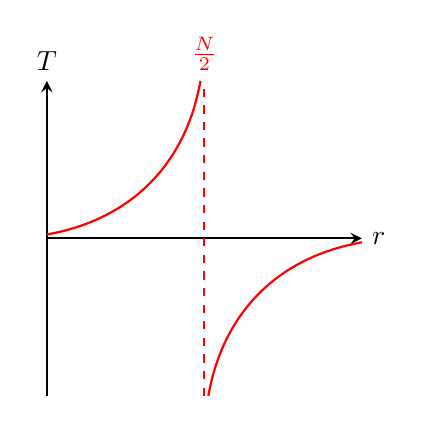
\begin{tikzpicture}
        \draw[thick, -stealth] (0,-2) -- (0,2) node[anchor=south] {$T$};
        \draw[thick, -stealth] (0,0) -- (4,0) node[anchor=west] {$r$};
        \draw[thick, red] (0,0.05) to[bend right=35] (1.95,2);
        \draw[thick,red] (2.05,-2) to[bend left=35] (4,-0.05);
        \draw[thick, dashed, red] (2,-2) -- (2,2) node[anchor=south] {$\frac{N}{2}$};
      \end{tikzpicture}\]

    Thanks to Andrew Binder for sharing me his \tikz code.

\end{solution}

\end{document}